% !TEX program = xelatex
% 由「TYC主图设计及进度」PPT 转换的 Beamer 模板：版式保留，内容与图均为占位符。
\documentclass[aspectratio=169,11pt]{beamer}
\usepackage[fontset=none]{ctex}
\usepackage{tikz,xcolor,graphicx,setspace,amsmath,amssymb,booktabs,array}
% 字体与原 PPT 一致：英文 Times New Roman；中文正文宋体(SimSun)；标题/封面中文微软雅黑(粗体)。
% 找不到时依次回退到系统里的其他中文字体。
\IfFontExistsTF{Times New Roman}{\setmainfont{Times New Roman}}{\setmainfont{TeX Gyre Termes}}
\IfFontExistsTF{SimSun}{\setCJKmainfont{SimSun}[AutoFakeBold=2]}
 {\IfFontExistsTF{Songti SC}{\setCJKmainfont{Songti SC}}
 {\IfFontExistsTF{Noto Serif CJK SC}{\setCJKmainfont{Noto Serif CJK SC}}
 {\IfFontExistsTF{AR PL UMing CN}{\setCJKmainfont{AR PL UMing CN}}{\setCJKmainfont{FandolSong}}}}}
\IfFontExistsTF{Microsoft YaHei}{\newCJKfontfamily\yahei{Microsoft YaHei}[AutoFakeBold=2]\setCJKsansfont{Microsoft YaHei}}
 {\IfFontExistsTF{SimHei}{\newCJKfontfamily\yahei{SimHei}[AutoFakeBold=2]\setCJKsansfont{SimHei}}
 {\IfFontExistsTF{PingFang SC}{\newCJKfontfamily\yahei{PingFang SC}\setCJKsansfont{PingFang SC}}
 {\IfFontExistsTF{Noto Sans CJK SC}{\newCJKfontfamily\yahei{Noto Sans CJK SC}\setCJKsansfont{Noto Sans CJK SC}}
 {\newCJKfontfamily\yahei{FandolHei}\setCJKsansfont{FandolHei}}}}}
\renewcommand{\familydefault}{\rmdefault}  % beamer 默认无衬线，改为 Times

%% ---------- 配色（取自原 PPT）----------
\definecolor{ttl}{HTML}{115399}   % 标题蓝
\definecolor{tag}{HTML}{C00000}   % 状态标签红
\definecolor{refc}{HTML}{3333B2}  % 参考文献字体色
\definecolor{phbg}{HTML}{EEF1F5}  % 占位框底色
\definecolor{phln}{HTML}{9AA5B4}
\setbeamercolor{normal text}{fg=black}
\setbeamercolor{background canvas}{bg=white}
\setbeamertemplate{navigation symbols}{}
\setbeamertemplate{itemize item}{\textcolor{ttl}{\tiny$\blacksquare$}}
\setbeamerfont{itemize/enumerate body}{size=\small}

%% ---------- 页面框架：顶部双线 + 标题 + 页脚线 ----------
\setbeamertemplate{headline}{}
\setbeamertemplate{footline}{%
  \begin{tikzpicture}[remember picture,overlay]
    \draw[ttl,line width=.6pt] ([xshift=.04\paperwidth,yshift=.08\paperheight]current page.south west)
      -- ([xshift=-.05\paperwidth,yshift=.08\paperheight]current page.south east);
    \node[anchor=east,font=\scriptsize\color{ttl}] at ([xshift=-.05\paperwidth,yshift=.04\paperheight]current page.south east){\insertframenumber};
  \end{tikzpicture}}
\setbeamertemplate{frametitle}{%
  \begin{tikzpicture}[remember picture,overlay]
    \draw[ttl,line width=1.2pt] ([xshift=.03\paperwidth,yshift=-.02\paperheight]current page.north west)
      -- ([xshift=-.02\paperwidth,yshift=-.02\paperheight]current page.north east);
    \draw[ttl,line width=.5pt] ([xshift=.03\paperwidth,yshift=-.09\paperheight]current page.north west)
      -- ([xshift=-.02\paperwidth,yshift=-.09\paperheight]current page.north east);
    \node[anchor=west,font=\yahei\bfseries\fontsize{15}{18}\selectfont\color{ttl}]
      at ([xshift=.03\paperwidth,yshift=-.055\paperheight]current page.north west){\insertframetitle};
  \end{tikzpicture}}

%% ---------- 占位符组件 ----------
% \PH{宽}{高}{说明}：图片占位框（正式用图时替换为 \includegraphics）
\newcommand{\PH}[3]{\begin{tikzpicture}
  \fill[phbg,draw=phln,dashed,line width=.6pt] (0,0) rectangle (#1,#2);
  \draw[phln,line width=.4pt] (0,0)--(#1,#2) (0,#2)--(#1,0);
  \node[fill=phbg,inner sep=3pt,font=\small\color{phln},align=center] at (#1/2,#2/2){#3};
\end{tikzpicture}}
% \Tag{状态}：红色状态标签（待修改 / 已修改 / 未完成）
\newcommand{\Tag}[1]{{\yahei\bfseries\color{tag}\large #1}}
% \FigCap{文字}：图注区（小字、两端对齐）
\newcommand{\FigCap}[1]{{\fontsize{8}{9.6}\selectfont #1\par}}
% 内容区绝对定位：\At{x}{y}{内容}，x,y 为占页面宽高的比例（左上角起）
\newcommand{\At}[3]{\begin{tikzpicture}[remember picture,overlay]
  \node[anchor=north west,inner sep=0] at ([xshift=#1\paperwidth,yshift=-#2\paperheight]current page.north west){#3};
\end{tikzpicture}}

\title{【项目名称占位】}
\author{【汇报人】}
\date{YYYY.MM.DD}

\setbeamertemplate{bibliography item}{\textcolor{refc}{\tiny$\blacksquare$}}
\begin{document}

%% ===== 1 封面：背景图取自原 PPT（cover.jpg）+ 半透明深色遮罩 + 白色文字 =====
\begin{frame}[plain]
  \begin{tikzpicture}[remember picture,overlay]
    \node[inner sep=0] at (current page.center){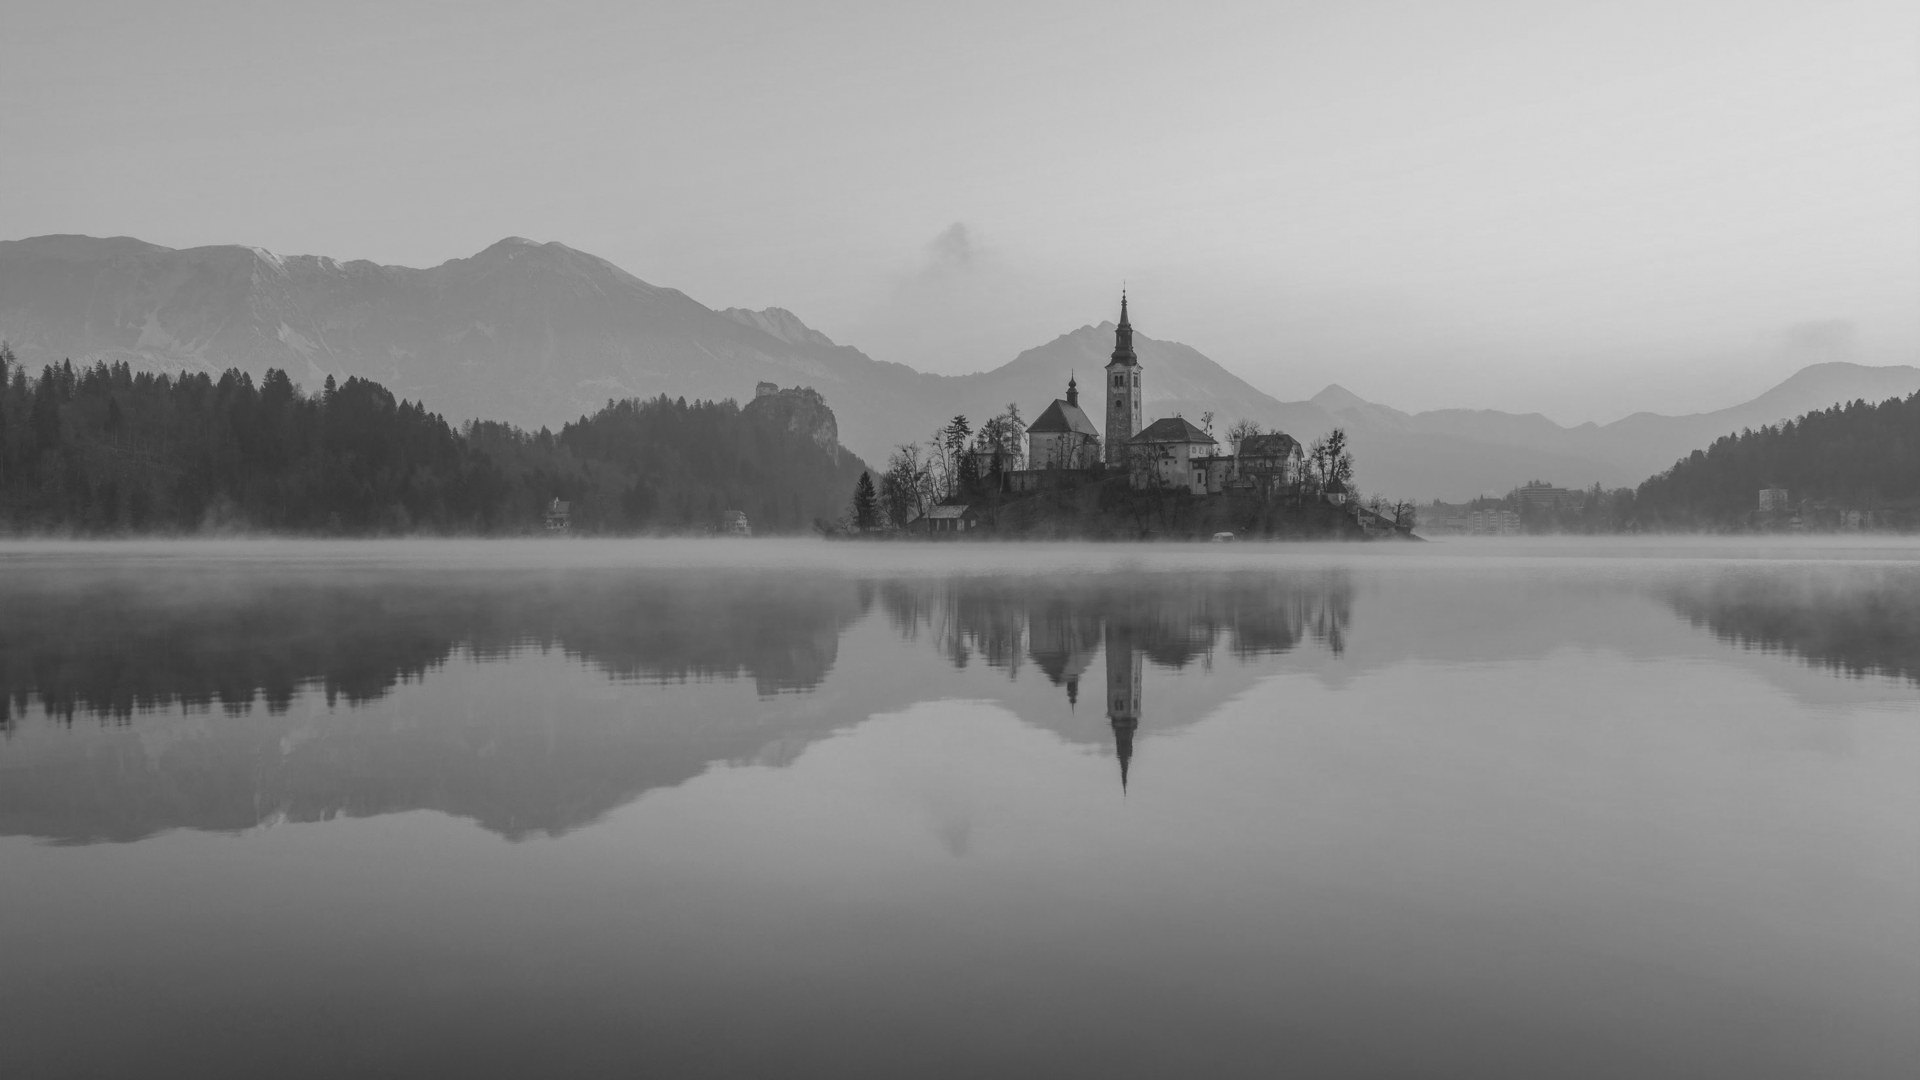
\includegraphics[width=\paperwidth,height=\paperheight]{cover.jpg}};
    \fill[black!95!white,opacity=.49] (current page.south west) rectangle (current page.north east);
    \foreach \y in {-.09,-.20}{\draw[white,line width=1pt] ([xshift=.1\paperwidth,yshift=\y\paperheight]current page.north west)
      -- ([xshift=-.08\paperwidth,yshift=\y\paperheight]current page.north east);}
    \draw[white,line width=1pt] ([xshift=.1\paperwidth,yshift=.15\paperheight]current page.south west)
      -- ([xshift=-.08\paperwidth,yshift=.15\paperheight]current page.south east);
    \node[font=\yahei\bfseries\fontsize{12}{14}\selectfont\color{white}] at ([yshift=-.145\paperheight]current page.north){项目名称占位};
    \node[text width=.8\paperwidth,align=center,font=\bfseries\fontsize{14}{17}\selectfont\color{white}] at ([yshift=-.30\paperheight]current page.north){English title placeholder: a long descriptive title of the project goes here};
    \node[text width=.8\paperwidth,align=center,font=\bfseries\fontsize{16}{19}\selectfont\color{white}] at ([yshift=-.48\paperheight]current page.north){中文标题占位：此处填写项目的中文题目};
    \node[text width=.8\paperwidth,align=center,font=\bfseries\fontsize{24}{28}\selectfont\color{white}] at ([yshift=-.70\paperheight]current page.north){副标题占位\\[4pt] YYYY.MM.DD};
  \end{tikzpicture}
\end{frame}

%% ===== 2 左图右字（图注）=====
\begin{frame}{Figure 1\quad 图标题占位}
  \At{.05}{.115}{\PH{.37\paperwidth}{.77\paperheight}{图 1 占位}}
  \At{.48}{.115}{\begin{minipage}{.46\paperwidth}
    \FigCap{\textbf{Figure 1.} 图注占位。\textbf{a,} 面板 a 说明占位。\textbf{b,} 面板 b 说明占位。\textbf{c,} 面板 c 说明占位。Lorem ipsum dolor sit amet, consectetur adipiscing elit, sed do eiusmod tempor incididunt ut labore et dolore magna aliqua.}
  \end{minipage}}
\end{frame}

%% ===== 3 左图右字（长图注）=====
\begin{frame}{Figure 2\quad 图标题占位}
  \At{.05}{.115}{\PH{.35\paperwidth}{.80\paperheight}{图 2 占位}}
  \At{.48}{.115}{\begin{minipage}{.46\paperwidth}
    \FigCap{\textbf{Figure 2.} 长图注占位。Lorem ipsum dolor sit amet, consectetur adipiscing elit, sed do eiusmod tempor incididunt ut labore et dolore magna aliqua. Ut enim ad minim veniam, quis nostrud exercitation ullamco laboris nisi ut aliquip ex ea commodo consequat. Duis aute irure dolor in reprehenderit in voluptate velit esse cillum dolore eu fugiat nulla pariatur.}
  \end{minipage}}
\end{frame}

%% ===== 4 全文字页：要点列表（含加粗小标题）=====
\begin{frame}{背景与目的}
  \begin{minipage}[t][.78\paperheight][t]{.92\paperwidth}
    \textbf{\color{ttl}\large 小节标题占位}\par\vspace{4pt}
    \begin{itemize}\setlength\itemsep{5pt}
      \item 要点一占位：Lorem ipsum dolor sit amet, consectetur adipiscing elit.
      \item 要点二占位：sed do eiusmod tempor incididunt ut labore et dolore magna aliqua.
      \begin{itemize}\item 子要点占位 \item 子要点占位\end{itemize}
      \item 要点三占位：ut enim ad minim veniam, quis nostrud exercitation ullamco.
    \end{itemize}
    \vspace{6pt}
    \textbf{\color{ttl}\large 段落小节占位}\par\vspace{4pt}
    \small Lorem ipsum dolor sit amet, consectetur adipiscing elit, sed do eiusmod tempor incididunt ut labore et dolore magna aliqua. Duis aute irure dolor in reprehenderit in voluptate velit esse cillum dolore eu fugiat nulla pariatur.
  \end{minipage}
\end{frame}

%% ===== 5 含公式页 =====
\begin{frame}{方法：公式}
  \begin{minipage}[t][.78\paperheight][t]{.92\paperwidth}
    \textbf{\color{ttl}\large 行内公式与独立公式}\par\vspace{4pt}
    占位说明文字，行内公式如 $F_{ST}=\dfrac{\pi_{B}-\pi_{W}}{\pi_{B}}$。
    \begin{equation}
      \text{Fold enrichment}=\frac{n_{\text{target}}/n_{\text{node}}}{N_{\text{target}}/N_{\text{total}}}
    \end{equation}
    \begin{align}
      S &= \frac{2\,f\,s}{f+s}, \label{eq:score}\\
      p &= \sum_{k\ge x}\frac{\binom{K}{k}\binom{N-K}{n-k}}{\binom{N}{n}}.
    \end{align}
    其中 $f$ 为占位变量 1，$s$ 为占位变量 2，$K,N,n$ 为占位参数。
  \end{minipage}
\end{frame}

%% ===== 6 含表格页（三线表）=====
\begin{frame}{结果：表格}
  \begin{minipage}[t][.78\paperheight][t]{.92\paperwidth}
    \centering
    {\small
    \begin{tabular}{l c c c c}
      \toprule
      组别占位 & 样本量 $n$ & 指标 A & 指标 B & $p$ 值 \\
      \midrule
      组 1 & 000 & 0.00 & 0.00 & $<0.001$ \\
      组 2 & 000 & 0.00 & 0.00 & 0.000 \\
      组 3 & 000 & 0.00 & 0.00 & 0.000 \\
      组 4 & 000 & 0.00 & 0.00 & 0.000 \\
      \bottomrule
    \end{tabular}}\par\vspace{6pt}
    {\footnotesize \textbf{Table 1.} 表注占位。Lorem ipsum dolor sit amet, consectetur adipiscing elit.\par}
  \end{minipage}
\end{frame}

%% ===== 7 参考文献页 =====
\begin{frame}{参考文献}
  \footnotesize\color{refc}
  \begin{thebibliography}{99}\setlength\itemsep{3pt}
    \bibitem{r1} Author A, Author B, Author C. Title of the first reference placeholder. \textit{Journal Name}. 2024;00(0):000--000.
    \bibitem{r2} Author D, Author E. Title of the second reference placeholder. \textit{Journal Name}. 2023;00(0):000--000.
    \bibitem{r3} Author F, et al. Title of the third reference placeholder. \textit{Journal Name}. 2022;00(0):000--000.
    \bibitem{r4} Author G, Author H. Title of the fourth reference placeholder. \textit{Journal Name}. 2021;00(0):000--000.
  \end{thebibliography}
\end{frame}

\end{document}
